\section{Evaluation}~\label{sec:eval}

{\bf Evaluation Method} We conduct our experiment with a set of large applications, e.g.,  those from the {\sf Dacapo} benchmark suite. 
The benchmarks are shown in Table. We compare our approach with the state-of-the-art technique proposed by Huang et al. As the capability of finding races depends on the monitored run, for fair comparison, we 
 apply both techniques to the same monitored run. Specifically, we use two threads in the monitored run as two threads are sufficient to manifest most of races~\cite{shanlu}. 

The {\sf Dacapo} relies on the reflection functionality to execute, which imposes challenges to static analysis and transformation. We apply the tool {\sf Tamiflex}~\cite{} to overcome the problems, which resolves the reflection using the classes observed in the dynamic run. The window size is 10000.


Our experiments and measurements 
were all conducted on an x86 64 Thinkpad W530 worksta- 
tion with eight 2.30GHz Intel Core i7-3610QM processors, 
16GB of RAM and 6M caches. The workstation runs version 12.04 of the Ubuntu Linux distribution, and has the Sun 
64-Bit 1.6.0\_26 Java virtual machine (JVM) installed~\footnote{Note that Sun JDK 1.7 does not support the transformation of dacapo applications with {\sf tamiflex}.}. 




\subsection{Scalability Issues}
Our approach suffers from scalability issues for two reasons. First, as we record local access events in the monitoring run,  the monitoring run takes long time, e.g., more than 2 hours, and our trace is typically large, e.g., at the GB level. To avoid the out of memory issue during the monitoring run, we store the event to the database on the fly, rather than storing them in a buffer. Besides, we terminate the monitoring run with a shutdown hook if it is beyond 30 minutes. Second,  the prediction phase needs to load the trace to memory, which easily causes out of memory problem. To solve the problem, we separate the analysis into several runs, each run restarting the JVM and resuming from the window of last run. Different runs communicate the window id using the external file. These runs are organized together automatically using the ant. The outputs of the files are merged into one summary finally. Besides, 


  


\begin{table}[htbp]
\caption{haha}
\begin{tabular}{|l|l|}
\hline
ad & fda \\ \hline
\multicolumn{1}{|r|}{1} & \multicolumn{1}{r|}{2} \\ \hline
\end{tabular}
\label{tb:ref}
\end{table}


\section{Case studies}
We manually inspect the reported races in small applications to gain better understanding about our approach. 

{\bf Relaxing the Inter-thread dependence\ } Figure~\ref{fig:relax1} demonstrates the relaxation of inter-thread dependence enabled by our approach. 
The code is from the benchmark {\sf bbuffer}, where the line number is marked. Huang et al.~\cite{} detects the race between line 291 and line 400, but fails to detect the race between line 294 and line 400. The reason is as follows. In the observation run, the execution follows the order,  lines 400, 291 and 294. For the event at line 294, its preceding branch at line 291 reads from line 400. Therefore, Huang et al.~\cite{}
 requires the predicted run to preserve the dependence between line 291 and line 400 so that line 291 reads exactly the same value and the branch takes the same branch decision. The dependence enforces the order constraint, $400 \rightarrow 291$, which further enforces the order $400\rightarrow 291 \rightarrow 294$.    Our approach does not require the existence of such dependence. Specifically, we allow line 291 to happen before line 400 in the predicted run as long as the value read by it leads to the same branch decision, which is true in this case.  As a result, there is no order constraint between line 294 and line 400, and the two forms a race. We re-replay such race  easily using the eclipse IDE breakpoints. 


 

\begin{figure}[htp]
\centering
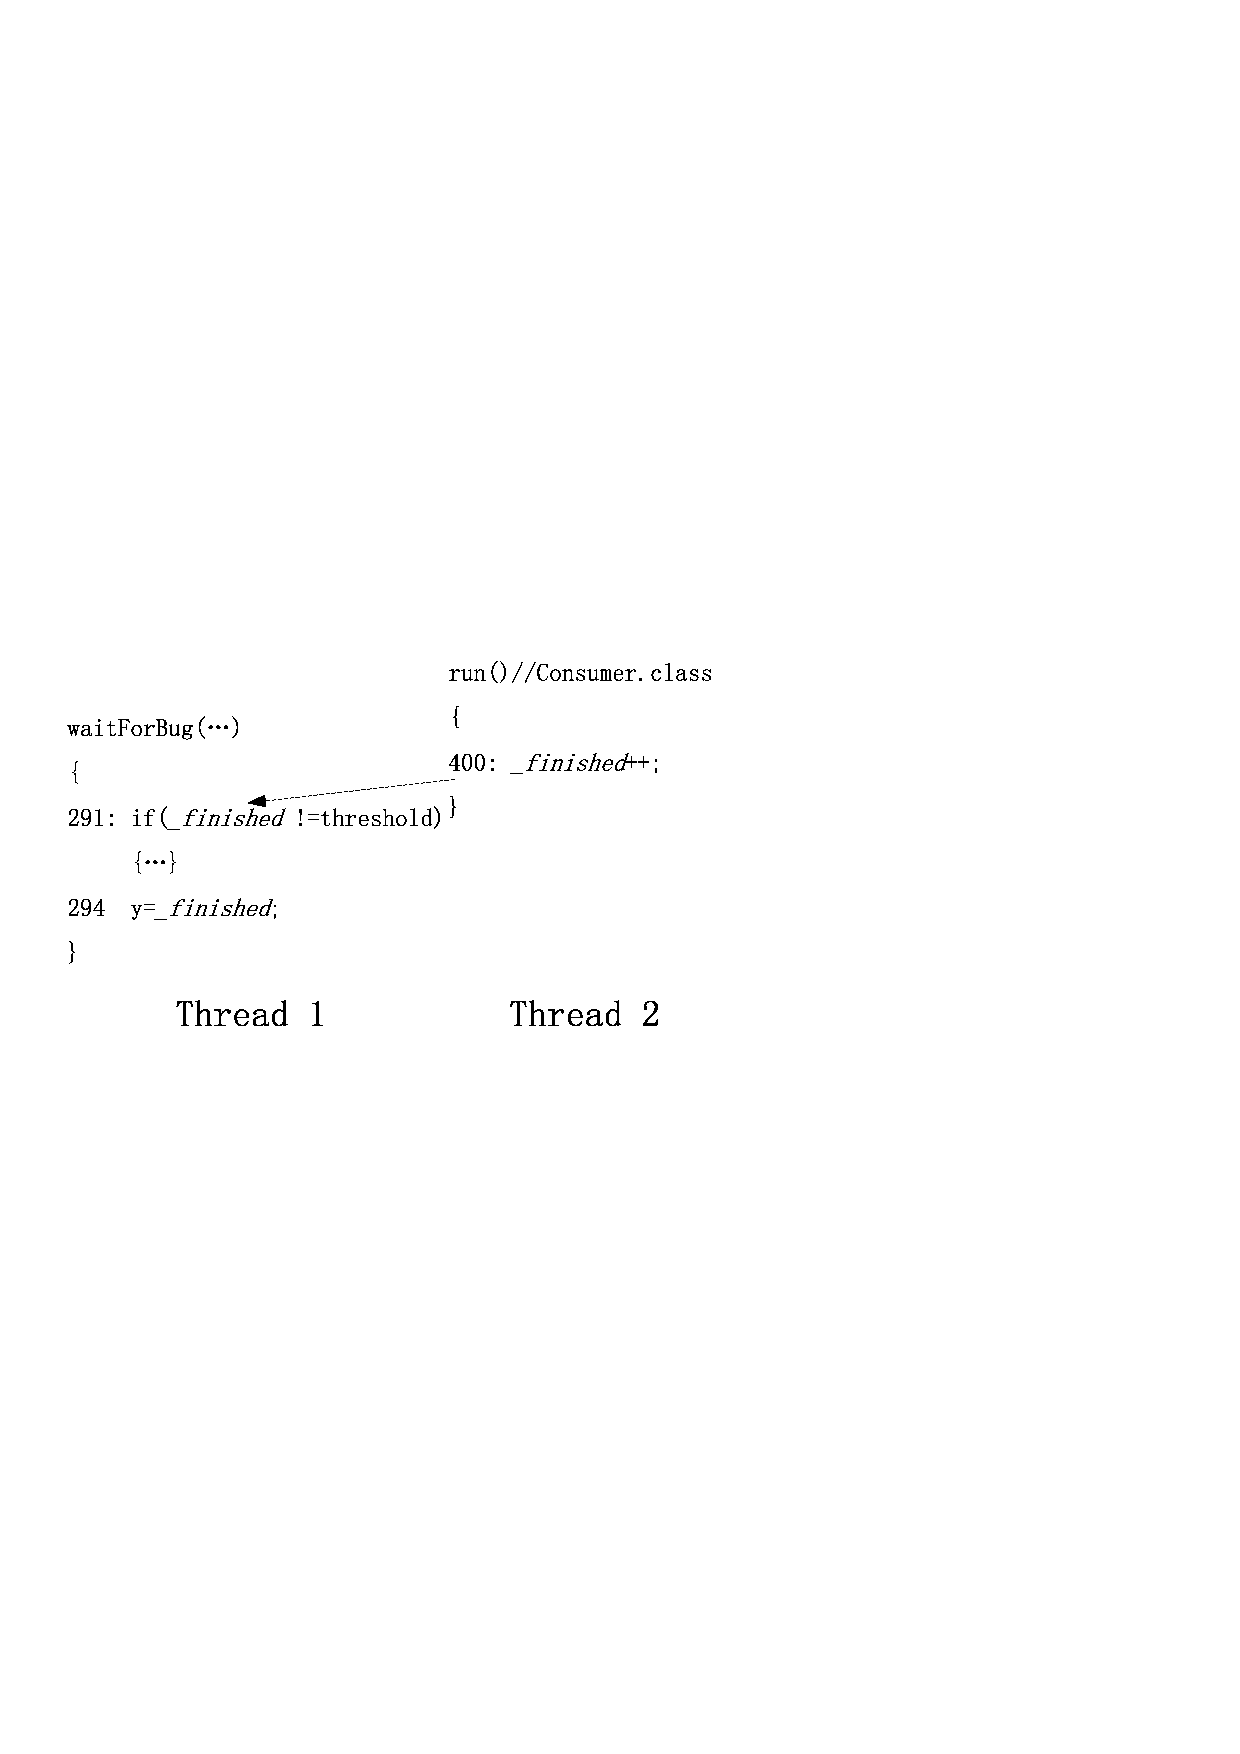
\includegraphics[scale=0.7]{cases/Visio-bbuffer.pdf}
\caption{Relaxation of Inter-thread dependence}\label{fig:relax1}
\end{figure}



\section{Validity Threat}
Java method can have 65535 bytecode instructions maximally. Therefore, we count the number of bytecode instructions inside each method, if the number exceeds 65525, we avoid instrumenting the method. The consequence is that, we will miss the races inside the method. In this case, we specify the variables read from the method to be equal to their concrete values in the constraints. THe constraint solver can proceed safely without being affected by such methods.

We do not support the boolean operations such as $\&$, bit operators $<<$, which contributes to most of our misses.



